%  LaTeX support: latex@mdpi.com 
%  For support, please attach all files needed for compiling as well as the log file, and specify your operating system, LaTeX version, and LaTeX editor.

\newcommand{\qsdpapertitle}{Planck Energy as Collapse Limit:
A Structural Interpretation of $E_P$ in Quantum Substrate Dynamics}
\newcommand{\qsdauthorname}{Michael Bush}
\newcommand{\qsdauthorinitials}{M.B.}
\newcommand{\qsdauthoremail}{mbush@haddentechnologies.com}
\newcommand{\qsdorcid}{0009-0003-9747-9109}
\newcommand{\qsdcorp}{Hadden Technologies Corporation}
\newcommand{\qsdkeywords}{Planck energy, Quantum Substrate Dynamics, coherence envelope, collapse limit, scalar pacing, gravitational compliance, phase-structured substrate, yield threshold, quantized offload, envelope rupture, Lorentz-invariant field theory, mass quantization, causal energy saturation, nonlinear collapse, inertial drag, structured emission, merger frustration, coherence recovery, quantized energy states}
\newcommand{\qsdmethodstatement}
{This manuscript was developed through a combination of theoretical derivation, substrate conservation modeling, and coherence-structured analysis. The expression for Planck energy was formulated by the author using first-principles substrate dynamics, with all mathematical relationships derived to preserve causal consistency, empirical falsifiability, and structural compatibility with both relativistic constraints and quantized behavior.}
\newcommand{\qsdabstract}
{In standard physics, Planck energy $E_P$ is often treated as a theoretical boundary marking the breakdown of classical descriptions, yet its structural origin remains obscure. In this work, we derive $E_P$ from first principles within the framework of Quantum Substrate Dynamics (QSD), a Lorentz-invariant field theory in which all physical action emerges from quantized coherence cycles within a conserved substrate. We show that $E_P$ reflects the \textit{maximum coherent energy density supportable by a single coherence envelope}, defined by the substrate’s transverse propagation limit $c_t$, curvature compliance $G$, and the geometric envelope scale $L_{\text{coh}}$. The result yields:
\[
E_P = \frac{c_t^4}{G} \cdot L_{\text{coh}}
\]
This expression reframes Planck energy as a structural \textit{yield threshold} of the substrate governing when collapse, rupture, or scalar offload becomes compulsory. We contextualize this result within the broader QSD framework, linking it to spectral serialization, causal pacing, and inertial drag. The collapse limit provides a physically grounded mechanism for high-energy emissions, mass-phase instability, and black hole merger frustration, and offers a falsifiable interpretation of the energetic limits observed in nature.}

%=================================================================
\documentclass[entropy,article,submit,pdftex,moreauthors]{Definitions/mdpi} 
%\documentclass[preprints,article,submit,pdftex,moreauthors]{Definitions/mdpi} 
% For posting an early version of this manuscript as a preprint, you may use "preprints" as the journal. Changing "submit" to "accept" before posting will remove line numbers.

% Below journals will use APA reference format:
% admsci, aieduc, behavsci, businesses, econometrics, economies, education, ejihpe, famsci, games, humans, ijcs, ijfs, journalmedia, jrfm, languages, psycholint, publications, tourismhosp, youth

% Below journals will use Chicago reference format:
% arts, genealogy, histories, humanities, jintelligence, laws, literature, religions, risks, socsci

%--------------------
% Class Options:
%--------------------
%----------
% journal
%----------
% Choose between the following MDPI journals:
% accountaudit, acoustics, actuators, addictions, adhesives, admsci, adolescents, aerobiology, aerospace, agriculture, agriengineering, agrochemicals, agronomy, ai, air, algorithms, allergies, alloys, amh, analytica, analytics, anatomia, anesthres, animals, antibiotics, antibodies, antioxidants, applbiosci, appliedchem, appliedmath, appliedphys, applmech, applmicrobiol, applnano, applsci, aquacj, architecture, arm, arthropoda, arts, asc, asi, astronomy, atmosphere, atoms, audiolres, automation, axioms, bacteria, batteries, bdcc, behavsci, beverages, biochem, bioengineering, biologics, biology, biomass, biomechanics, biomed, biomedicines, biomedinformatics, biomimetics, biomolecules, biophysica, biosensors, biosphere, biotech, birds, blockchains, bloods, blsf, brainsci, breath, buildings, businesses, cancers, carbon, cardiogenetics, catalysts, cells, ceramics, challenges, chemengineering, chemistry, chemosensors, chemproc, children, chips, cimb, civileng, cleantechnol, climate, clinbioenerg, clinpract, clockssleep, cmd, cmtr, coasts, coatings, colloids, colorants, commodities, complications, compounds, computation, computers, condensedmatter, conservation, constrmater, cosmetics, covid, crops, cryo, cryptography, crystals, csmf, ctn, curroncol, cyber, dairy, data, ddc, dentistry, dermato, dermatopathology, designs, devices, diabetology, diagnostics, dietetics, digital, disabilities, diseases, diversity, dna, drones, dynamics, earth, ebj, ecm, ecologies, econometrics, economies, education, eesp, ejihpe, electricity, electrochem, electronicmat, electronics, encyclopedia, endocrines, energies, eng, engproc, ent, entomology, entropy, environments, epidemiologia, epigenomes, esa, est, famsci, fermentation, fibers, fintech, fire, fishes, fluids, foods, forecasting, forensicsci, forests, fossstud, foundations, fractalfract, fuels, future, futureinternet, futureparasites, futurepharmacol, futurephys, futuretransp, galaxies, games, gases, gastroent, gastrointestdisord, gastronomy, gels, genealogy, genes, geographies, geohazards, geomatics, geometry, geosciences, geotechnics, geriatrics, glacies, grasses, greenhealth, gucdd, hardware, hazardousmatters, healthcare, hearts, hemato, hematolrep, heritage, higheredu, highthroughput, histories, horticulturae, hospitals, humanities, humans, hydrobiology, hydrogen, hydrology, hygiene, idr, iic, ijerph, ijfs, ijgi, ijmd, ijms, ijns, ijpb, ijt, ijtm, ijtpp, ime, immuno, informatics, information, infrastructures, inorganics, insects, instruments, inventions, iot, j, jal, jcdd, jcm, jcp, jcs, jcto, jdad, jdb, jeta, jfb, jfmk, jimaging, jintelligence, jlpea, jmahp, jmmp, jmms, jmp, jmse, jne, jnt, jof, joitmc, joma, jop, jor, journalmedia, jox, jpbi, jpm, jrfm, jsan, jtaer, jvd, jzbg, kidney, kidneydial, kinasesphosphatases, knowledge, labmed, laboratories, land, languages, laws, life, lights, limnolrev, lipidology, liquids, literature, livers, logics, logistics, lubricants, lymphatics, machines, macromol, magnetism, magnetochemistry, make, marinedrugs, materials, materproc, mathematics, mca, measurements, medicina, medicines, medsci, membranes, merits, metabolites, metals, meteorology, methane, metrics, metrology, micro, microarrays, microbiolres, microelectronics, micromachines, microorganisms, microplastics, microwave, minerals, mining, mmphys, modelling, molbank, molecules, mps, msf, mti, multimedia, muscles, nanoenergyadv, nanomanufacturing, nanomaterials, ncrna, ndt, network, neuroglia, neurolint, neurosci, nitrogen, notspecified, nursrep, nutraceuticals, nutrients, obesities, oceans, ohbm, onco, oncopathology, optics, oral, organics, organoids, osteology, oxygen, parasites, parasitologia, particles, pathogens, pathophysiology, pediatrrep, pets, pharmaceuticals, pharmaceutics, pharmacoepidemiology, pharmacy, philosophies, photochem, photonics, phycology, physchem, physics, physiologia, plants, plasma, platforms, pollutants, polymers, polysaccharides, populations, poultry, powders, preprints, proceedings, processes, prosthesis, proteomes, psf, psych, psychiatryint, psychoactives, psycholint, publications, purification, quantumrep, quaternary, qubs, radiation, reactions, realestate, receptors, recycling, regeneration, religions, remotesensing, reports, reprodmed, resources, rheumato, risks, robotics, rsee, ruminants, safety, sci, scipharm, sclerosis, seeds, sensors, separations, sexes, signals, sinusitis, siuj, skins, smartcities, sna, societies, socsci, software, soilsystems, solar, solids, spectroscj, sports, standards, stats, std, stresses, surfaces, surgeries, suschem, sustainability, symmetry, synbio, systems, tae, targets, taxonomy, technologies, telecom, test, textiles, thalassrep, therapeutics, thermo, timespace, tomography, tourismhosp, toxics, toxins, transplantology, transportation, traumacare, traumas, tropicalmed, universe, urbansci, uro, vaccines, vehicles, venereology, vetsci, vibration, virtualworlds, viruses, vision, waste, water, wem, wevj, wild, wind, women, world, youth, zoonoticdis

%---------
% article
%---------
% The default type of manuscript is "article", but can be replaced by: 
% abstract, addendum, article, benchmark, book, bookreview, briefcommunication, briefreport, casereport, changes, clinicopathologicalchallenge, comment, commentary, communication, conceptpaper, conferenceproceedings, correction, conferencereport, creative, datadescriptor, discussion, entry, expressionofconcern, extendedabstract, editorial, essay, erratum, fieldguide, hypothesis, interestingimages, letter, meetingreport, monograph, newbookreceived, obituary, opinion, proceedingpaper, projectreport, reply, retraction, review, perspective, protocol, shortnote, studyprotocol, supfile, systematicreview, technicalnote, viewpoint, guidelines, registeredreport, tutorial,  giantsinurology, urologyaroundtheworld
% supfile = supplementary materials

%----------
% submit
%----------
% The class option "submit" will be changed to "accept" by the Editorial Office when the paper is accepted. This will only make changes to the frontpage (e.g., the logo of the journal will get visible), the headings, and the copyright information. Also, line numbering will be removed. Journal info and pagination for accepted papers will also be assigned by the Editorial Office.

%------------------
% moreauthors
%------------------
% If there is only one author the class option oneauthor should be used. Otherwise use the class option moreauthors.

%---------
% pdftex
%---------
% The option pdftex is for use with pdfLaTeX. Remove "pdftex" for (1) compiling with LaTeX & dvi2pdf (if eps figures are used) or for (2) compiling with XeLaTeX.

%=================================================================
% MDPI internal commands - do not modify
\firstpage{1} 
\makeatletter 
\setcounter{page}{\@firstpage} 
\makeatother
\pubvolume{1}
\issuenum{1}
\articlenumber{0}
\pubyear{2025}
\copyrightyear{2025}
%\externaleditor{Firstname Lastname} % More than 1 editor, please add `` and '' before the last editor name
\datereceived{ } 
\daterevised{ } % Comment out if no revised date
\dateaccepted{ } 
\datepublished{ } 
%\datecorrected{} % For corrected papers: "Corrected: XXX" date in the original paper.
%\dateretracted{} % For retracted papers: "Retracted: XXX" date in the original paper.
\hreflink{https://doi.org/} % If needed use \linebreak
%\doinum{}
%\pdfoutput=1 % Uncommented for upload to arXiv.org
%\CorrStatement{yes}  % For updates
%\longauthorlist{yes} % For many authors that exceed the left citation part

%=================================================================
% Add packages and commands here. The following packages are loaded in our class file: fontenc, inputenc, calc, indentfirst, fancyhdr, graphicx, epstopdf, lastpage, ifthen, float, amsmath, amssymb, lineno, setspace, enumitem, mathpazo, booktabs, titlesec, etoolbox, tabto, xcolor, colortbl, soul, multirow, microtype, tikz, totcount, changepage, attrib, upgreek, array, tabularx, pbox, ragged2e, tocloft, marginnote, marginfix, enotez, amsthm, natbib, hyperref, cleveref, scrextend, url, geometry, newfloat, caption, draftwatermark, seqsplit
% cleveref: load \crefname definitions after \begin{document}

\usepackage{tikz}
\usetikzlibrary{angles, quotes}
\usepackage{pgfplots}
\pgfplotsset{compat=1.17}

\usepackage{amsmath}
\usetikzlibrary{positioning}
%=================================================================
% Please use the following mathematics environments: Theorem, Lemma, Corollary, Proposition, Characterization, Property, Problem, Example, ExamplesandDefinitions, Hypothesis, Remark, Definition, Notation, Assumption
%% For proofs, please use the proof environment (the amsthm package is loaded by the MDPI class).

%=================================================================
% Full title of the paper (Capitalized)
\Title{\qsdpapertitle}


% MDPI internal command: Title for citation in the left column
\TitleCitation{Title}

% Author Orchid ID: enter ID or remove command
\newcommand{\orcidauthorA}{\qsdorcid} % Add \orcidA{} behind the author's name
%\newcommand{\orcidauthorB}{0000-0000-0000-000X} % Add \orcidB{} behind the author's name

% Authors, for the paper (add full first names)
\Author{\qsdauthorname $^{1}$\orcidA{}}

%\longauthorlist{yes}

% MDPI internal command: Authors, for metadata in PDF
\AuthorNames{\qsdauthorname}

% MDPI internal command: Authors, for citation in the left column, only choose below one of them according to the journal style
% If this is a Chicago style journal 
% (arts, genealogy, histories, humanities, jintelligence, laws, literature, religions, risks, socsci): 
% Lastname, Firstname, Firstname Lastname, and Firstname Lastname.

% If this is a APA style journal 
% (admsci, behavsci, businesses, econometrics, economies, education, ejihpe, games, humans, ijfs, journalmedia, jrfm, languages, psycholint, publications, tourismhosp, youth): 
% Lastname, F., Lastname, F., \& Lastname, F.

% If this is a ACS style journal (Except for the above Chicago and APA journals, all others are in the ACS format): 
% Lastname, F.; Lastname, F.; Lastname, F.
\isAPAStyle{%
       \AuthorCitation{Lastname, F., Lastname, F., \& Lastname, F.}
         }{%
        \isChicagoStyle{%
        \AuthorCitation{Lastname, Firstname, Firstname Lastname, and Firstname Lastname.}
        }{
        \AuthorCitation{Lastname, F.; Lastname, F.; Lastname, F.}
        }
}

% Affiliations / Addresses (Add [1] after \address if there is only one affiliation.)
\address{%
$^{1}$ \quad \qsdcorp; \qsdauthoremail\\
%$^{2}$ \quad Affiliation 2; e-mail@e-mail.com
}

% Contact information of the corresponding author
\corres{Correspondence: \qsdauthoremail (\qsdauthorinitials)}

% Current address and/or shared authorship
%\firstnote{Shiloh, IL: Independent Researcher.}  % Current address should not be the same as any items in the Affiliation section.
%\secondnote{These authors contributed equally to this work.}
% The commands \thirdnote{} till \eighthnote{} are available for further notes

%\simplesumm{} % Simple summary

%\conference{} % An extended version of a conference paper


% Abstract (Do not insert blank lines, i.e. \\) 
\abstract{\qsdabstract}

% Keywords
\keyword{\qsdkeywords} 

% The fields PACS, MSC, and JEL may be left empty or commented out if not applicable
%\PACS{J0101}
%\MSC{}
%\JEL{}

%%%%%%%%%%%%%%%%%%%%%%%%%%%%%%%%%%%%%%%%%%
% Only for the journal Diversity
%\LSID{\url{http://}}

%%%%%%%%%%%%%%%%%%%%%%%%%%%%%%%%%%%%%%%%%%
% Only for the journal Applied Sciences
%\featuredapplication{Authors are encouraged to provide a concise description of the specific application or a potential application of the work. This section is not mandatory.}
%%%%%%%%%%%%%%%%%%%%%%%%%%%%%%%%%%%%%%%%%%

%%%%%%%%%%%%%%%%%%%%%%%%%%%%%%%%%%%%%%%%%%
% Only for the journal Data
%\dataset{DOI number or link to the deposited data set if the data set is published separately. If the data set shall be published as a supplement to this paper, this field will be filled by the journal editors. In this case, please submit the data set as a supplement.}
%\datasetlicense{License under which the data set is made available (CC0, CC-BY, CC-BY-SA, CC-BY-NC, etc.)}

%%%%%%%%%%%%%%%%%%%%%%%%%%%%%%%%%%%%%%%%%%
% Only for the journal BioTech, Fishes, Neuroimaging and Toxins
%\keycontribution{The breakthroughs or highlights of the manuscript. Authors can write one or two sentences to describe the most important part of the paper.}

%%%%%%%%%%%%%%%%%%%%%%%%%%%%%%%%%%%%%%%%%%
% Only for the journal Encyclopedia
%\encyclopediadef{For entry manuscripts only: please provide a brief overview of the entry title instead of an abstract.}

%%%%%%%%%%%%%%%%%%%%%%%%%%%%%%%%%%%%%%%%%%
% Only for the journal Advances in Respiratory Medicine, Future, Sensors and Smart Cities
%\addhighlights{yes}
%\renewcommand{\addhighlights}{%
%
%\noindent This is an obligatory section in ``Advances in Respiratory Medicine'', ``Future'', ``Sensors'' and ``Smart Cities”, whose goal is to increase the discoverability and readability of the article via search engines and other scholars. Highlights should not be a copy of the abstract, but a simple text allowing the reader to quickly and simplified find out what the article is about and what can be cited from it. Each of these parts should be devoted up to 2~bullet points.\vspace{3pt}\\
%\textbf{What are the main findings?}
% \begin{itemize}[labelsep=2.5mm,topsep=-3pt]
% \item First bullet.
% \item Second bullet.
% \end{itemize}\vspace{3pt}
%\textbf{What is the implication of the main finding?}
% \begin{itemize}[labelsep=2.5mm,topsep=-3pt]
% \item First bullet.
% \item Second bullet.
% \end{itemize}
%}

%%%%%%%%%%%%%%%%%%%%%%%%%%%%%%%%%%%%%%%%%%
\begin{document}
%%%%%%%%%%%%%%%%%%%%%%%%%%%%%%%%%%%%%%%%%%
% The order of the section titles is different for some journals. Please refer to the "Instructions for Authors” on the journal homepage.

%%%%%%%%%%%%%%%%%%%%%%%%%%%%%%%%%%%%%%%%%%
\section{Introduction}
%%%%%%%%%%%%%%%%%%%%%%%%%%%%%%%%%%%%%%%%%%

Planck-scale constants such as \( \hbar \), \( \ell_P \), and \( E_P \) appear across quantum mechanics, relativity, and field theory as natural units that demarcate physical limits. While these constants define scales of action, length, and energy, their physical origin remains abstract. In most frameworks, \( E_P \)---the Planck energy---is introduced dimensionally, as a derived combination of fundamental constants. Yet its interpretation often remains speculative: is it a maximum energy? A threshold for quantum gravity? A boundary where classical theory breaks down?

Quantum Substrate Dynamics (QSD) \cite{bush2025} provides a structural framework in which Planck energy arises not from dimensional analysis alone, but from the causal and geometric constraints of a coherence-bound substrate. In QSD, energy is not an independent quantity, but the measurable consequence of coherent offload within a Lorentz-invariant medium. Coherence structures---mass-phase configurations---can only persist, move, or interact if they remain recoverable within bounded regions of the substrate. These regions are defined by the coherence envelope \( L_{\text{coh}}^3 \), which governs the minimal support volume for causally valid structure.

In this context, Planck energy is reinterpreted as the structural collapse limit: the maximum coherent energy density that the substrate can support within a single coherence envelope before scalar collapse becomes inevitable. The expression
\[
E_P = \frac{c_t^4}{G} \cdot L_{\text{coh}}
\]
is not a theoretical maximum in the abstract, but a physical saturation threshold---the point at which internal curvature and tension exceed the substrate’s ability to maintain phase-locked structure. Beyond this limit, coherent mass-phase configurations cannot persist and must offload energy into the surrounding substrate, resulting in emission, decay, or geometric disintegration.

This paper develops the structural interpretation of \( E_P \) as a collapse threshold within QSD. We derive its form from first principles, link it to the previously established coherence envelope, and explore its role in governing the limits of mass stability, waveform persistence, and energetic containment. The reinterpretation of Planck energy as a causal boundary---rather than a speculative frontier---grounds it within a physical model of coherence, recovery, and structural failure. The result is a testable, geometrically constrained, and causally meaningful explanation for one of the most fundamental constants in modern physics.

While this work introduces a novel substrate-based framework, it acknowledges the long-standing efforts to understand collapse, coherence, and the role of physical constants in both classical and quantum contexts. The behavior of quantized emission from saturating wave envelopes has been explored in nonlinear optical systems \cite{boyd2008}, and decoherence has been widely discussed as a mechanism for classical emergence from quantum substrates \cite{zurek2003}. The philosophical and dimensional status of constants such as $\hbar$ and $G$ continues to evolve across multiple theoretical frameworks \cite{duff2002}. The present formulation does not directly rely on these treatments, but recognizes them as part of the broader effort to contextualize quantization, coherence, and physical law.


%%%%%%%%%%%%%%%%%%%%%%%%%%%%%%%%%%%%%%%%%%
\section{Materials and Methods}
%%%%%%%%%%%%%%%%%%%%%%%%%%%%%%%%%%%%%%%%%%
\qsdmethodstatement

In support of the editorial process, generative AI tools—specifically OpenAI's ChatGPT (version GPT-4o, 2025)—were used to assist in:
\begin{itemize}
    \item Generating illustrative figures based on the author’s conceptual framework, with iterative refinement to ensure fidelity to the substrate-based dynamics of the model,
    \item Researching, validating, and cross-referencing related scientific concepts to improve accuracy, contextual alignment, and clarity,
    \item Summarizing and formatting externally sourced material already selected by the author.
\end{itemize}

No original theoretical contributions were generated by the AI system; all scientific claims, hypotheses, derivations, and interpretations were authored and reviewed by the human researcher. The use of ChatGPT is disclosed in alignment with journal policy for transparency in the writing process.

%%%%%%%%%%%%%%%%%%%%%%%%%%%%%%%%%%%%%%%%%%
%\section{Results}

%%%%%%%%%%%%%%%%%%%%%%%%%%%%%%%%%%%%%%%%%%
\section{Discussion}
%%%%%%%%%%%%%%%%%%%%%%%%%%%%%%%%%%%%%%%%%%
%%%%%%%%%%%%%%%%%%%%%%%%%%%%%%%%%%%%%%%%%%%
\subsection{The Collapse Threshold as a Physical Limit}
%%%%%%%%%%%%%%%%%%%%%%%%%%%%%%%%%%%%%%%%%%%
In the standard view of high-energy physics, Planck energy $E_P$ is regarded as a symbolic upper bound---an extrapolated scale at which quantum and gravitational effects are presumed to unify, often without a clearly defined physical mechanism. Within the Quantum Substrate Dynamics (QSD) framework, however, this threshold gains a specific structural meaning: it is the \textit{maximum coherent energy supportable by a single substrate envelope} before rupture occurs.

\begin{equation}
E_P = \frac{c_t^4}{G} \cdot L_{\text{coh}}
\end{equation}

This expression is not speculative; it follows directly from substrate conservation and geometry. It reflects a \textit{physical saturation point}: the total energy that a coherence envelope of size $L_{\text{coh}}$ can carry before its internal phase structure exceeds the substrate’s curvature compliance. In this model, collapse does not occur because of mathematical singularities or undefined field behavior---it occurs because \textit{the substrate can no longer reconfigure fast enough to maintain coherence} under the load.

This yield behavior is not continuous or reversible. Once the threshold is surpassed:
\begin{itemize}
  \item The envelope destabilizes,
  \item Scalar pacing is broken,
  \item Energy is offloaded either as quantized emission (e.g., radiation) or as structural rupture (e.g., TIGB or gravitational-wave precursor).
\end{itemize}

Unlike in general relativity, where black hole collapse leads to undefined conditions hidden behind event horizons, QSD provides a mechanism for \textit{observable collapse precursors and coherent emission boundaries}. Collapse is not an abstract divergence---it is a phase response to \textit{substrate saturation}. The system fails not because of infinite density, but because the region \textit{can no longer store coherence structure within the allowed pacing cycle}. Scalar recovery is outmatched by the energy stored in the transverse envelope.

The collapse threshold thus represents \textit{a causal limit on the substrate’s capacity to maintain phase continuity}, not a fundamental breakdown of theory. It defines a point beyond which \textit{no internal structure can remain stable without reorganizing or offloading}. This offload may be serial (burst emissions), layered (rebound shells), or catastrophic (coherence fracture), depending on the local topology and pacing gradients.

As such, the Planck energy in QSD is no longer a dimensional construct---it is a \textit{directly interpretable physical limit} tied to geometric, causal, and recoverable substrate behavior. It is falsifiable through collapse structure, spectral emission patterns, and the presence of quantized ejection events at known energy densities.
%%%%%%%%%%%%%%%%%%%%%%%%%%%%%%%%%%%%%%%%%%%%
\subsection{Toward a Mathematical Formalism for Collapse Dynamics}

The preceding sections have shown that Planck energy in QSD represents the maximum energy that a coherence envelope of size $L_{\text{coh}}$ can sustain before rupture, defined by the saturation of scalar pacing and transverse energy support. To model the dynamic behavior of this collapse more formally, we now outline a minimal mathematical framework that captures the essential features of envelope evolution near the collapse limit.

\subsubsection{Envelope Energy Evolution}

Let \( \rho(x, t) \) denote the local coherence tension density in a region of the substrate.\footnote{In QSD, \( \rho(x,t) \) denotes the \textit{local coherence tension density}, not the classical energy density derived from a stress–energy tensor. It represents the substrate’s phase compression state, which governs mass-phase persistence, scalar wave propagation, and tension reconfiguration capacity.} The total energy contained within a coherence envelope of spatial extent $L_{\text{coh}}$ is then:


\begin{equation}
E(t) = \int_{V} \rho(x,t)^2 \, d^3x
\end{equation}

where $V$ is the coherence-supporting volume at time $t$. As transverse energy is injected or accumulated into the region, $\rho$ increases and approaches a maximum supportable value $\rho_{\text{crit}}$ set by the structural yield threshold:

\begin{equation}
\rho_{\text{crit}} \approx \frac{E_P}{L_{\text{coh}}^3}
\end{equation}

This provides a dynamic criterion: when the local energy density $\rho(x,t)$ exceeds this threshold, the envelope is no longer recoverable and will yield.

\subsubsection{Collapse Condition and Recovery Lag}

The scalar pacing constraint defines a recovery interval:

\begin{equation}
t_P = \frac{L_{\text{coh}}}{c_s}
\end{equation}

A collapse event is triggered when the energy injection or internal reconfiguration rate exceeds the recoverable pacing of the scalar mode:

\begin{equation}
\frac{dE}{dt} > \frac{E_P}{t_P} = \frac{c_t^4}{G}
\end{equation}

This defines a local collapse rate ceiling: any process that delivers energy faster than this limit must result in scalar rupture or yield.

\subsubsection{Envelope Instability Growth}

We may define an instability field $\Phi(x,t)$ which evolves under coherence strain. Its dynamics obey a driven nonlinear diffusion equation of the form:

\begin{equation}
\frac{\partial \Phi}{\partial t} = D_{\text{coh}} \nabla^2 \Phi + \alpha \rho(x,t)^2 - \beta \Phi
\end{equation}

where:
\begin{itemize}
  \item $D_{\text{coh}}$ is a coherence diffusivity constant (analogous to how fast phase stress propagates),
  \item $\alpha$ couples local energy density to rupture likelihood,
  \item $\beta$ models substrate damping or recovery.
\end{itemize}

Collapse onset occurs when $\Phi(x,t) \to \Phi_{\text{crit}}$, corresponding to a coherence fracture front that propagates through the envelope. Once rupture is triggered locally, the collapse front propagates causally through the envelope as a scalar phase discontinuity. This front expands outward from the saturation point, limited by the scalar recovery speed $c_s$, and reshapes the coherence configuration as it passes. This resembles domain wall rupture in condensed matter systems or mode-locked pulse fronts in optical media. The spatial spread is not instantaneous, but layered and structured, allowing partial offload in concentric or asymmetric bursts depending on local curvature, see Figure \ref{fig:collapse_front}.

\begin{figure}[H]
  \centering
  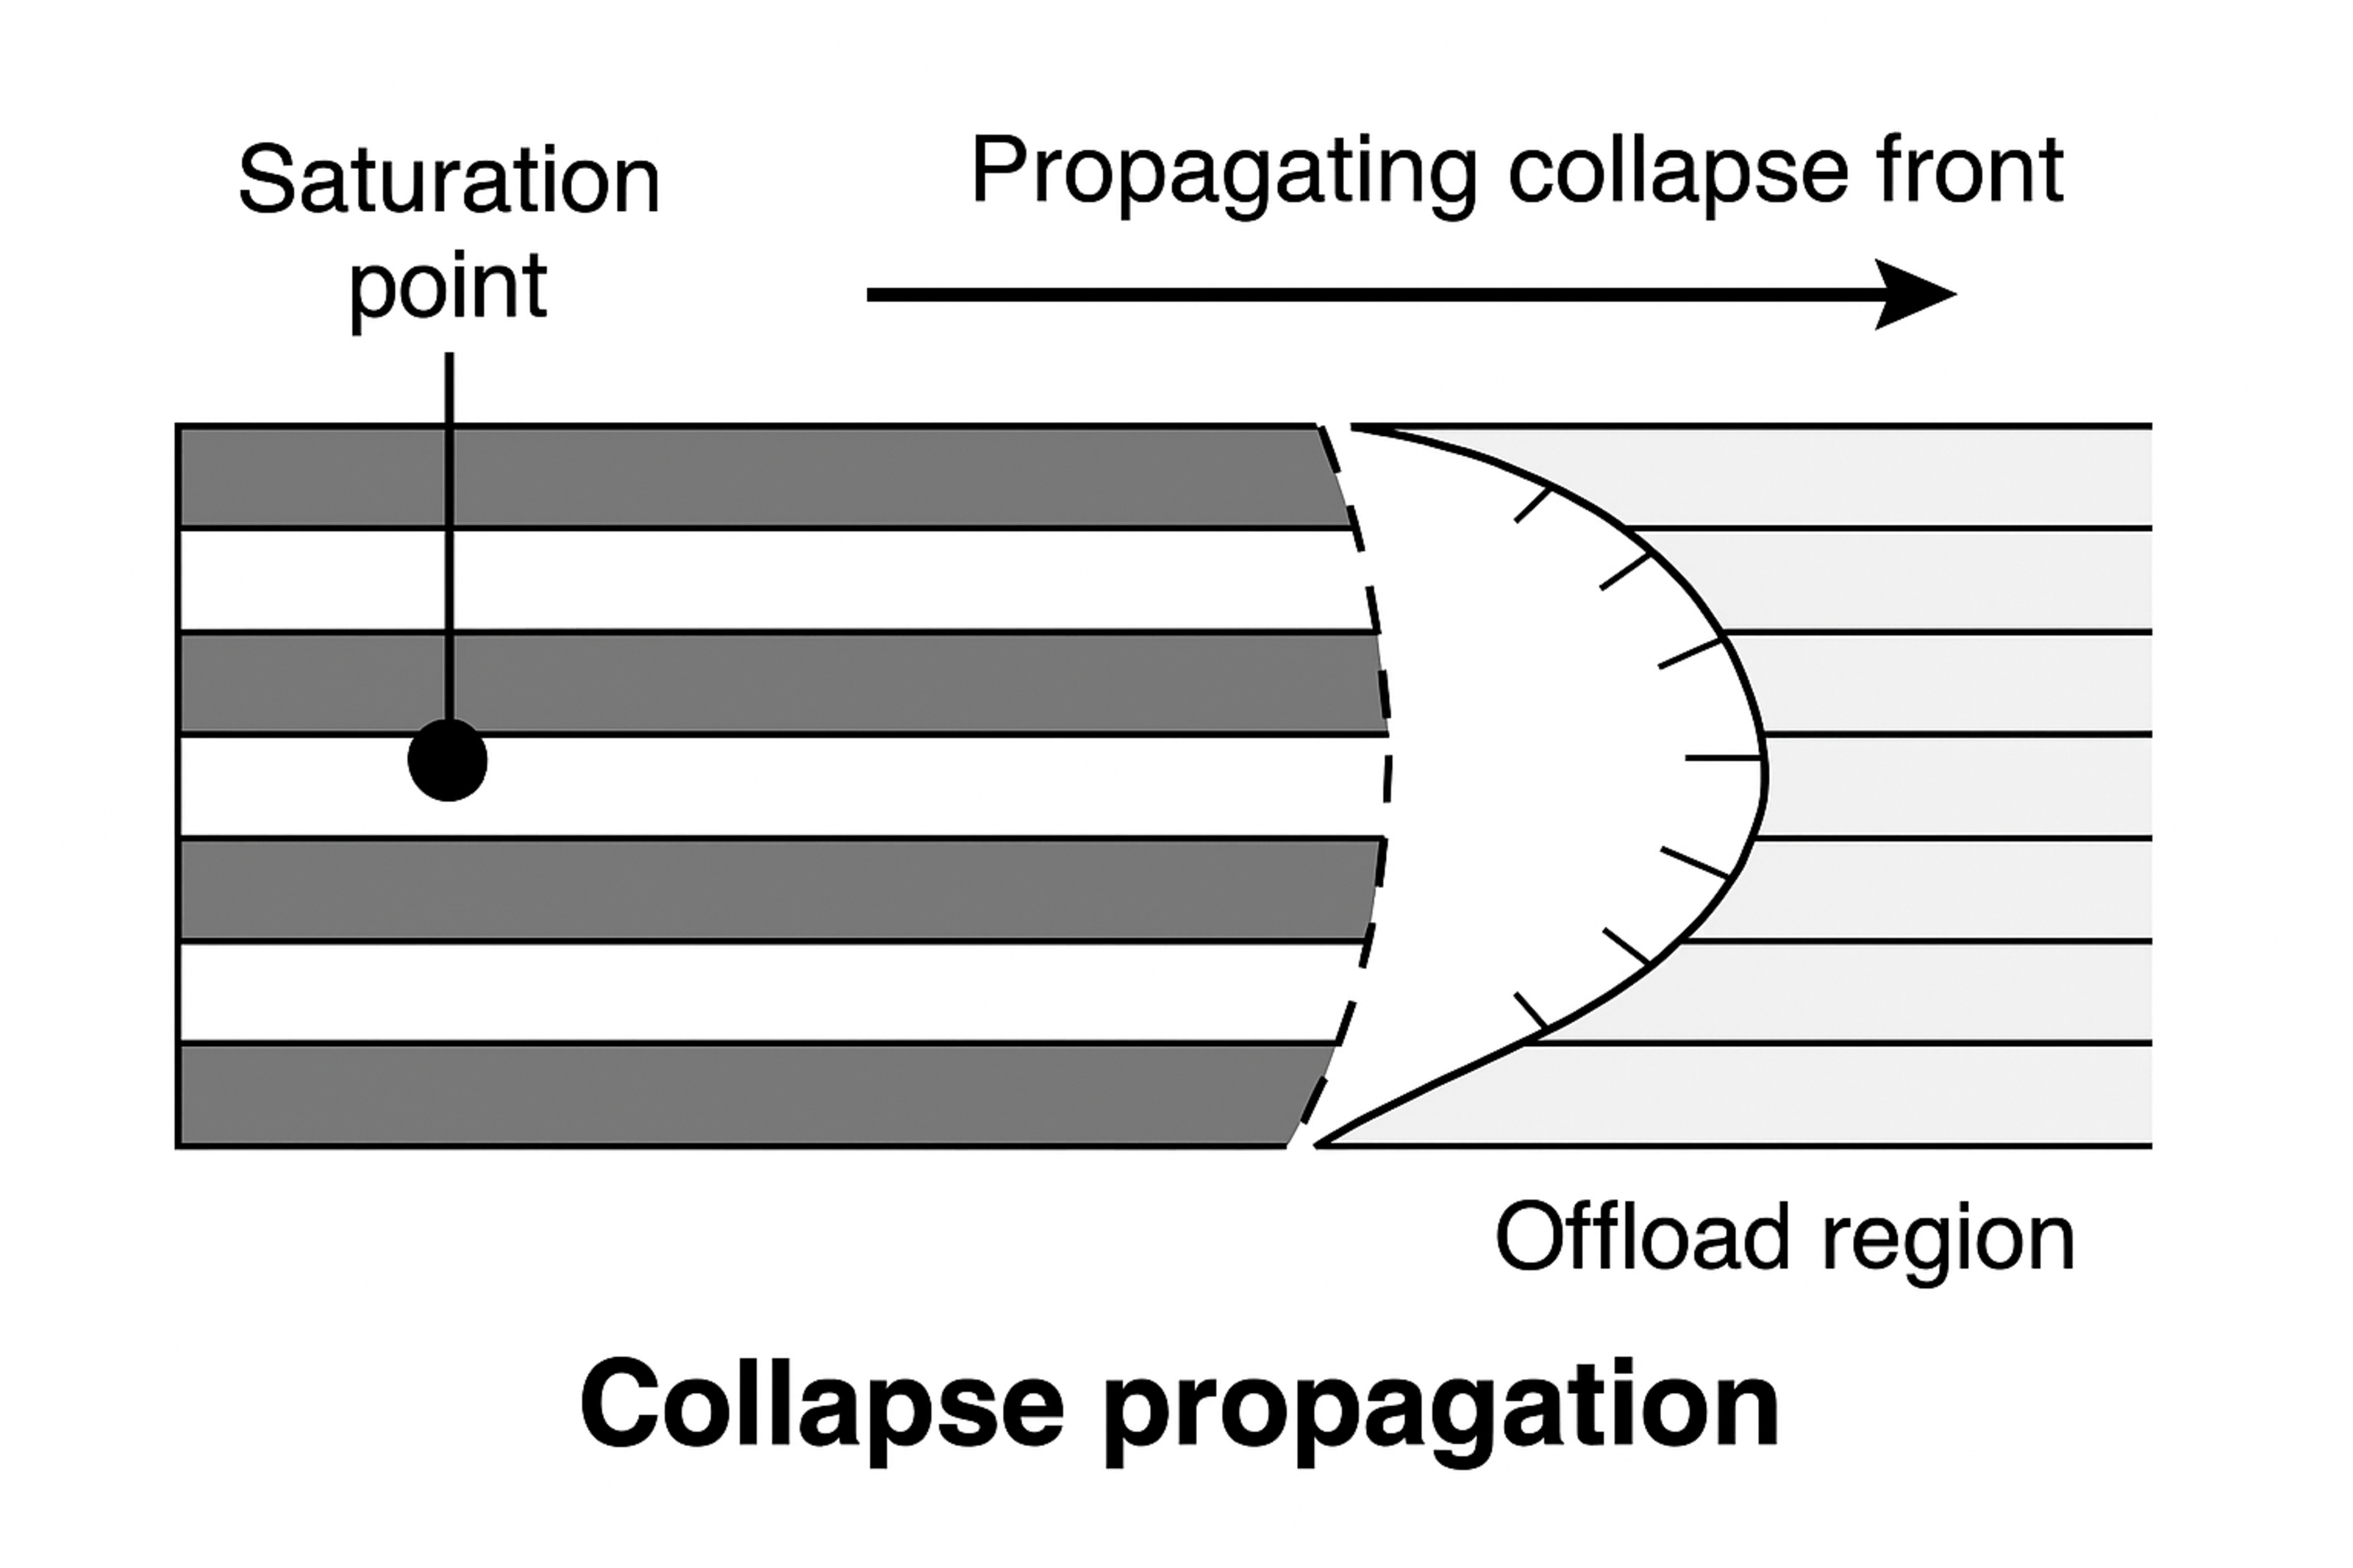
\includegraphics[width=0.75\linewidth]{figures/collapse.pdf}
  \caption{Collapse front propagation from a coherence-saturated region. The rupture front expands causally at the scalar pacing speed $c_s$, redistributing stored energy and triggering structural offload. The curvature of the rupture boundary reflects directional strain and recovery geometry.}
  \label{fig:collapse_front}
\end{figure}

\subsubsection{Post-Rupture Recovery and Memory Effects}

Whether rupture originates at the outer boundary of a coherence envelope or within its interior, the affected substrate region enters a scalar recovery phase. During this interval, no new coherent mass-phase structure can form until local phase alignment is restored. The recovery timescale is bounded below by the scalar pacing limit:

\begin{equation}
t_P = \frac{L_{\text{coh}}}{c_s},
\end{equation}

but full structural reset may require multiple cycles depending on rupture intensity, envelope topology, and residual tension gradients.

We model the local recovery state with a coherence restoration function $R(x,t)$, normalized such that $R = 0$ represents a ruptured region and $R = 1$ represents full recovery of local substrate coherence. A simple first-order temporal model can be written as:

\begin{equation}
\frac{\partial R}{\partial t} = \frac{1}{\tau_r} (1 - R) - \Gamma(x,t),
\end{equation}

where:
\begin{itemize}
  \item $\tau_r$ is the characteristic recovery time, typically $\gtrsim t_P$,
  \item $\Gamma(x,t)$ is a damping or inhibition term representing lingering scalar strain or residual interference from prior collapse.
\end{itemize}

In the absence of secondary rupture or active inhibition ($\Gamma \rightarrow 0$), the solution approaches exponential recovery:

\begin{equation}
R(t) = 1 - e^{-t/\tau_r},
\end{equation}

indicating that even after causal pacing permits substrate reuse, full structural coherence is only asymptotically restored. In systems with partial rupture or nonlinear recoil, $\Gamma(x,t)$ may remain non-zero for extended intervals, delaying envelope reuse.

Because the coherence substrate is causal and continuous, the rupture location—whether at the core, shell, or mid-envelope—only determines the geometry of the recovery front, not its physics. The recovery field $R(x,t)$ evolves locally, ensuring that both surface-triggered and interior-origin collapse obey the same pacing and memory constraints.

Importantly, the substrate retains partial memory of prior coherence geometry during this process. This memory may manifest as structural bias for future envelope formation, preferred symmetry axes, or altered rupture thresholds in subsequent offload events. These effects resemble residual topologies in post-collapse domain realignment, and may explain observable coherence imprinting in burst emissions or collapse echoes.



\subsubsection{Emission Profile and Envelope Offload}

Once rupture begins, energy is released in quantized bursts, structured by the coherence geometry of the mass-phase knot. The offload power can be approximated as:

\begin{equation}
P_{\text{offload}}(t) = \frac{dE_{\text{emit}}}{dt} \approx \gamma \cdot \frac{E_P}{t_P} \cdot f(t)
\end{equation}

where $f(t)$ is a normalized burst profile shaped by envelope asymmetry and scalar delay gradients, and $\gamma \leq 1$ accounts for partial rupture or phased re-emission.

This function determines the observable signature of the event: its rise time, spectral distribution, and recurrence behavior.

\subsubsection{Summary and Future Directions}

This formalism is not yet a complete set of QSD field equations, but it demonstrates how core substrate variables---energy density, pacing speed, coherence diffusivity, and structural geometry---can be coupled to model collapse and offload dynamics. Extensions of this model may include:

\begin{itemize}
  \item Nonlinear recovery gating with temporal hysteresis,
  \item Geometric dependence of $L_{\text{coh}}$ under envelope deformation,
  \item Tensorial modeling of phase stress and directional rupture propagation.
\end{itemize}

Ultimately, this framework aims to replace singularity-based collapse models with a structurally recoverable, quantized, and falsifiable description of mass-phase envelope failure under coherent substrate limits.
%%%%%%%%%%%%%%%%%%%%%%%%%%%%%%%%%%%%%%%%%%%%
\subsection{Explicit Treatment of \texorpdfstring{$L_{\text{coh}}$}{Lcoh} Quantization}

The coherence envelope length $L_{\text{coh}}$ plays a central role in determining the energy capacity, pacing constraints, and collapse behavior of mass-phase structures in QSD. While previous sections have treated $L_{\text{coh}}$ as a continuous variable to establish general saturation dynamics, the substrate’s structural properties suggest that only a discrete set of envelope configurations are physically stable. This leads naturally to a form of \textit{geometric mass quantization}.


\subsubsection{Quantized Envelope Modes}

In a conserved coherence substrate, the envelope must maintain:
\begin{enumerate}
  \item Internal phase symmetry,
  \item Sufficient scalar pacing to prevent rupture,
  \item Boundary continuity across wavefronts.
\end{enumerate}

These conditions constrain the allowed spatial forms of stable coherence envelopes to standing-wave-like structures that satisfy both geometric closure and causal pacing. As a result, only certain values of $L_{\text{coh}}$ support persistent, phase-locked mass-phase configurations.

We denote these quantized envelope modes as:

\begin{equation}
L_n = n \cdot L_0,
\end{equation}

where $L_0$ is the minimum coherence length scale supported by the substrate (often set by the structural Planck length), and $n \in \mathbb{N}$ defines the envelope mode number.

Each quantized $L_n$ defines a distinct energy limit:

\begin{equation}
E_{P,n} = \frac{c_t^4}{G} \cdot L_n = \hbar \cdot \frac{c_s}{L_n}
\end{equation}

This relationship suggests that different particle or mass states correspond to stable coherence configurations occupying distinct $L_n^3$ envelopes, each with its own energy support, pacing interval, and rupture threshold.

These allowable envelope configurations are visualized in Figure~\ref{fig:envelope_modes}, which shows discrete standing-wave modes constrained within the same coherence boundary $L_n$. Only these quantized modes can persist as recoverable mass-phase structures within the substrate.

\begin{figure}[H]
  \centering
  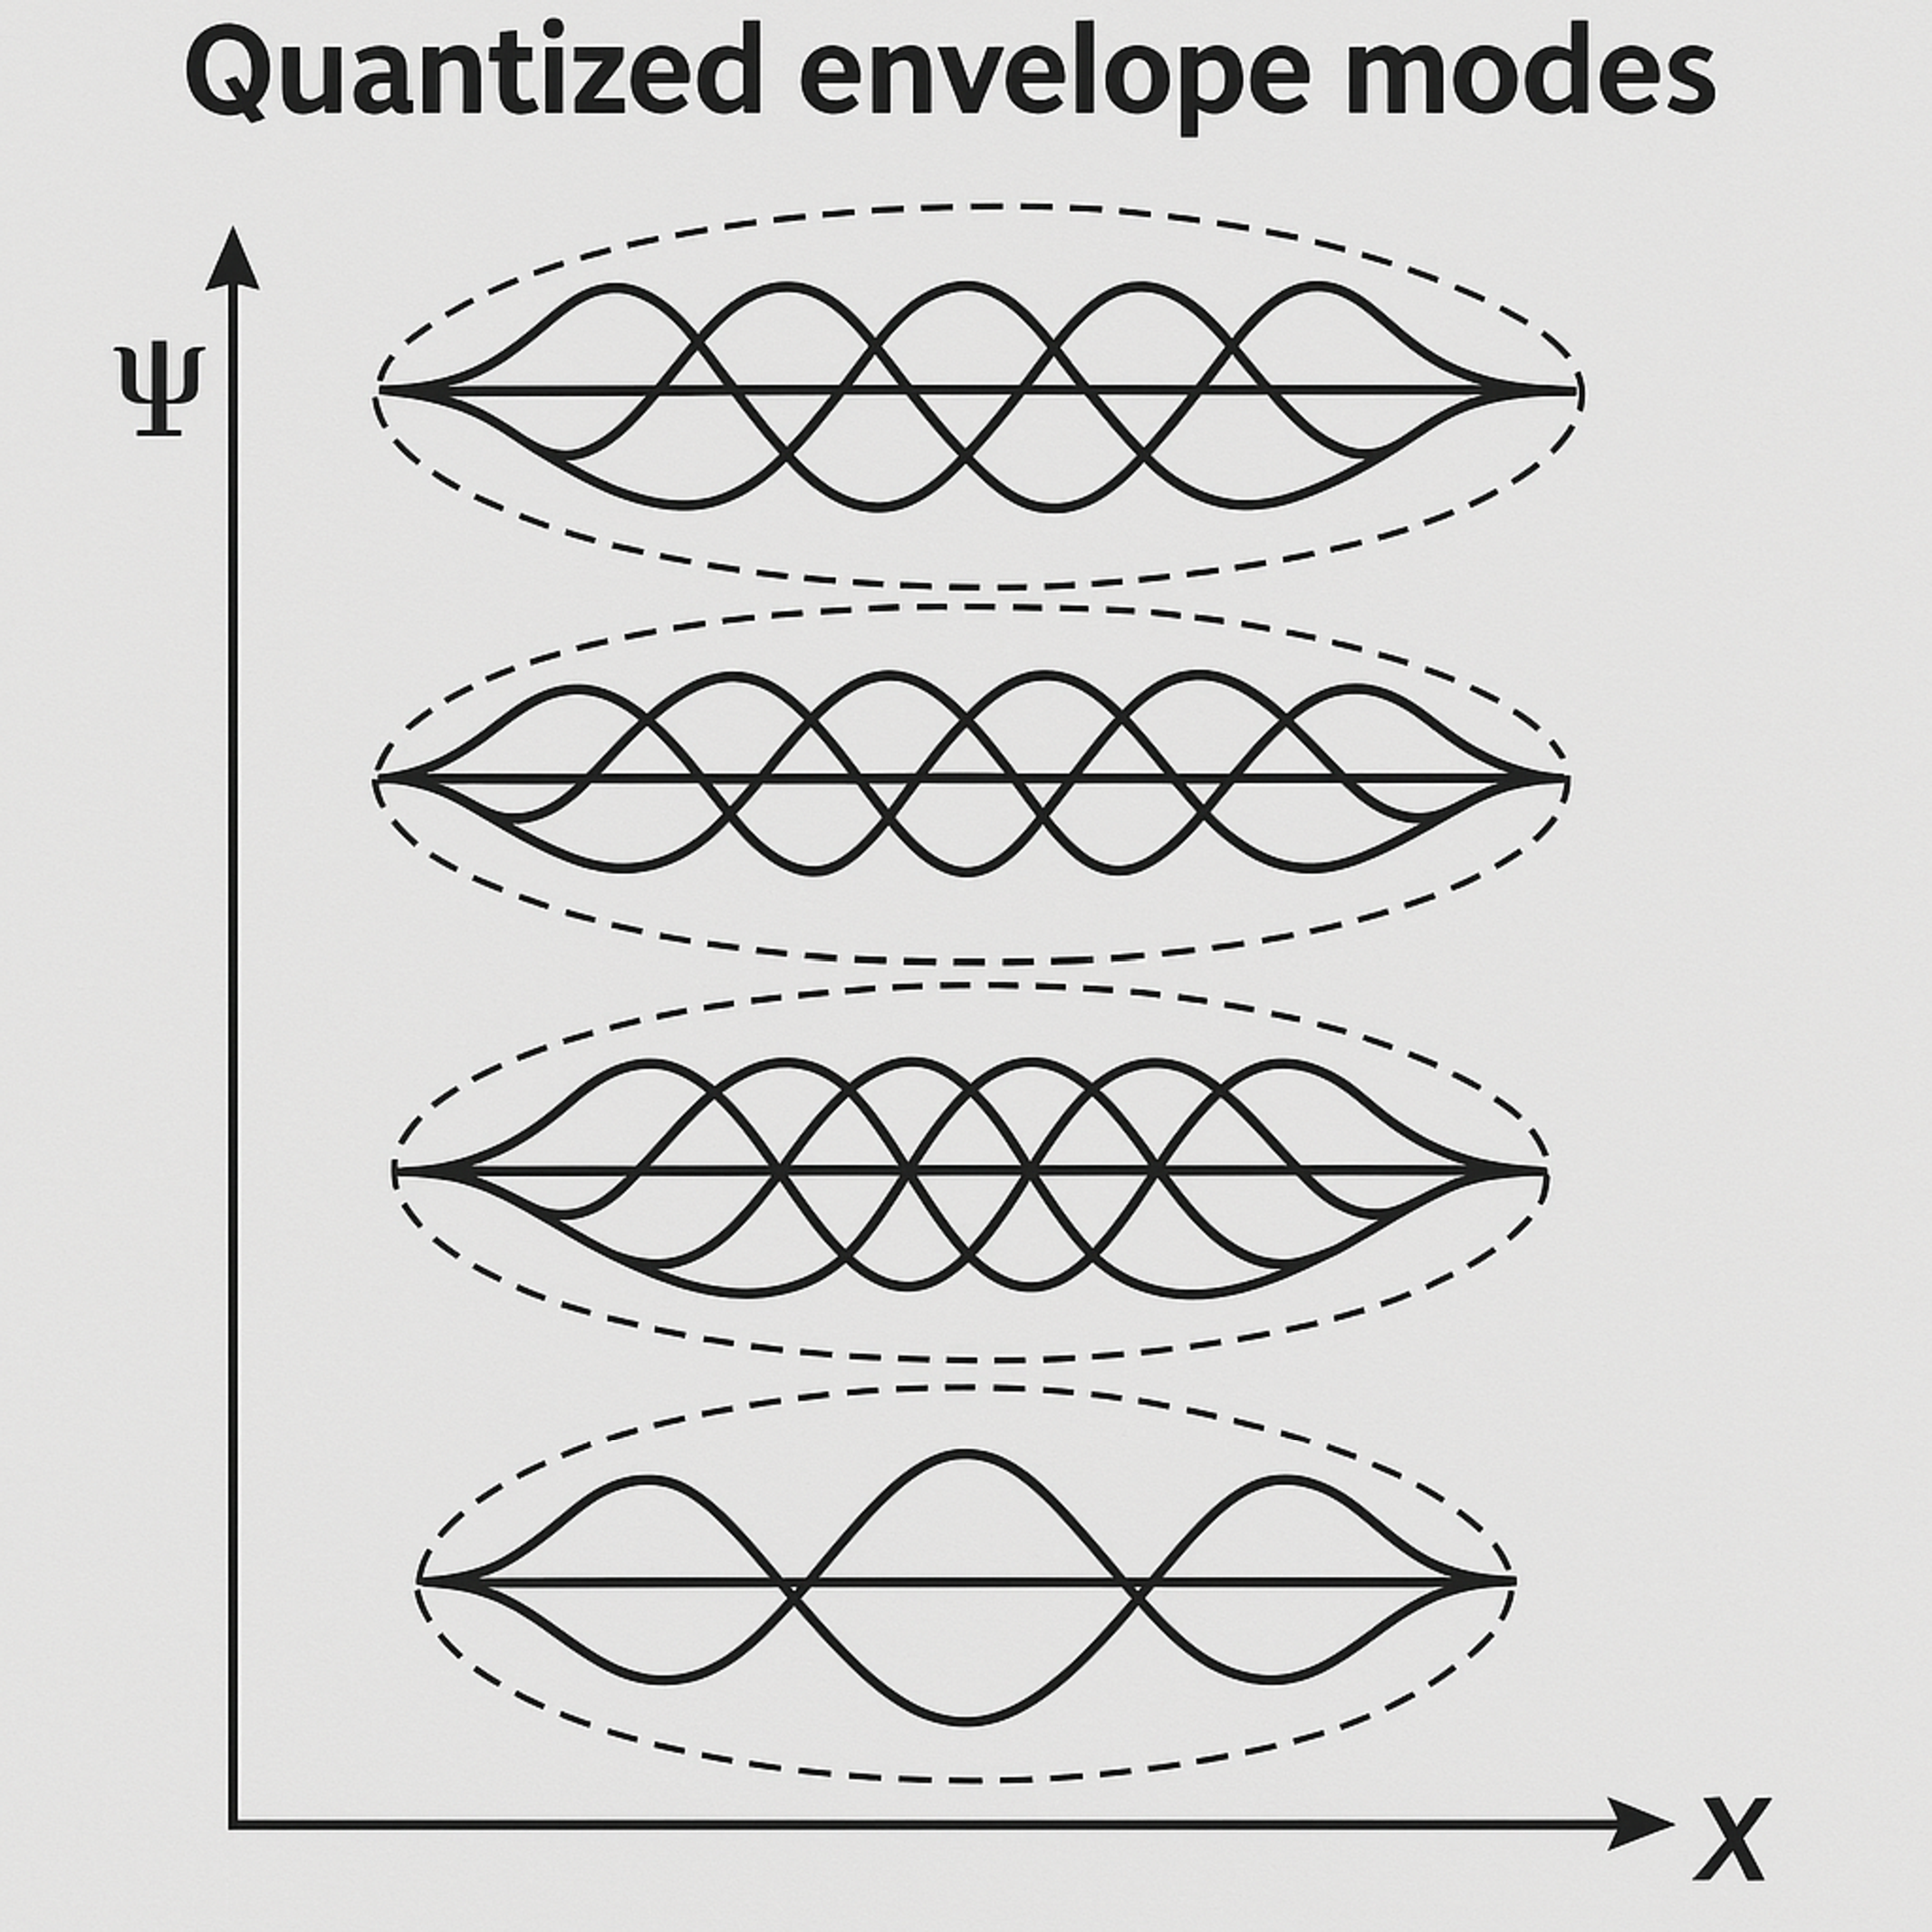
\includegraphics[width=0.65\linewidth]{figures/envelope.pdf}
  \caption{Quantized envelope modes illustrating allowable standing-wave configurations within a coherence domain. Each mode corresponds to a stable mass-phase structure and is associated with a quantized energy level $E_n = \hbar \cdot \frac{n c_s}{L_{\text{coh}}}$.}
  \label{fig:envelope_modes}
\end{figure}


\subsubsection{Implications for Mass and Energy Discreteness}

Mass in QSD is not a pointlike quantity but a persistent, structured phase configuration within a coherence volume. Quantization of $L_{\text{coh}}$ therefore implies quantization of:
\begin{itemize}
  \item Supported energy values (mass–energy equivalence),
  \item Recovery pacing (Planck time variants),
  \item Emission thresholds (burst energy spectra),
  \item Stability domains (permitted particle geometries).
\end{itemize}

This creates a discrete lattice of allowed structural mass states. Unstable or non-permitted $L_{\text{coh}}$ values either fail to form, decay into lower modes, or offload energy until a stable envelope configuration is reached.

\subsubsection{Observational and Experimental Relevance}

Quantization of $L_{\text{coh}}$ introduces a testable structure to the spectrum of mass and energy. If each stable matter state corresponds to a quantized coherence envelope, we expect:
\begin{itemize}
  \item Mass thresholds and cutoffs at regular geometric intervals,
  \item Spectral emission features during collapse events tied to envelope mode transitions,
  \item A finite spectrum of stable phase knots matching observed particle states.
\end{itemize}

This provides a mechanism to explain why only certain mass values occur in nature and why high-energy events emit in structured, quantized bursts.

\subsubsection{Summary}

In QSD, $L_{\text{coh}}$ is not a continuously tunable parameter but a geometrically constrained and causally gated structure. Only discrete envelope modes can maintain phase coherence under recoverable substrate conditions. This leads naturally to mass quantization as a geometric effect, offering a substrate-level explanation for particle spectra, energy levels, and coherent emission thresholds.

%%%%%%%%%%%%%%%%%%%%%%%%%%%%%%%%%%%%%%%%%%%%
\subsection{Structural Origins of \texorpdfstring{$G$}{G}: Compliance, Not Constant}

In classical physics, Newton’s gravitational constant $G$ is treated as a fixed coupling parameter—a universal scaling factor inserted into the gravitational law without explanation of its physical origin. Within the QSD framework, however, $G$ is revealed to be a \textit{compliance factor} of the substrate: a structural property that reflects how easily the substrate yields to curvature imposed by local phase tension.

This reinterpretation is rooted in the structural derivation of Planck’s constant $\hbar$ from substrate geometry. In QSD, $\hbar$ emerges from the offload structure of a coherence envelope, governed by modal propagation speeds and coherence size:

\begin{equation}
\hbar = \frac{c_t^4}{c_s} \cdot \frac{L_{\text{coh}}^2}{G}
\end{equation}

Rearranging, we obtain a structural expression for $G$:

\begin{equation}
G = \frac{c_t^4}{c_s} \cdot \frac{L_{\text{coh}}^2}{\hbar}
\end{equation}

Here, $c_t$ is the transverse coherence propagation speed (governing spatial energy transfer), $c_s$ is the scalar recovery speed, which governs how fast the substrate resets its internal coherence after an energy offload or collapse event. It sets the minimum interval between successive energy transfers within a coherence envelope.
, $L_{\text{coh}}$ is the coherence support length, and $\hbar$ is the minimum offload unit—a structural action quantum. This shows that $G$ is not a fixed coupling inserted externally, but a \textit{derived ratio} from internal substrate properties.

\medskip
This has several critical implications:

\begin{itemize}
  \item \textbf{Geometric dependence}: $G$ scales with $L_{\text{coh}}^2$, the coherence area. In compact, saturated systems (e.g., near black hole cores), $L_{\text{coh}}$ compresses, leading to a reduced effective $G$—i.e., tighter curvature compliance.
  \item \textbf{Causal pacing control}: The recovery speed $c_s$ limits how fast the substrate can support scalar reconfiguration. Slower pacing increases the apparent compliance, modulating $G$ in time-dependent systems.
  \item \textbf{Modal embedding}: The transverse propagation speed $c_t$ governs how rapidly coherence tension spreads spatially, and appears raised to the fourth power—highlighting its dominant role in determining gravitational stiffness.
\end{itemize}

This expression also explains why $G$ appears constant under typical conditions: in most systems, $L_{\text{coh}}$, $c_t$, and $c_s$ remain approximately stable across moderate curvature regimes. However, QSD predicts that $G$ will vary across extreme curvature gradients, such as in neutron stars, galactic halos, or high-strain merger zones.

Furthermore, $G$ acts analogously to an \textit{elastic modulus} in material science—a measure of how much phase curvature the substrate tolerates per unit energy tension. Systems with higher phase gradient curvature (strong coherence strain) experience a “stiffer” substrate, corresponding to a lower effective $G$.

This structural derivation also aligns with the Planck energy expression in QSD:

\begin{equation}
E_P = \frac{c_t^4}{G} \cdot L_{\text{coh}}
\end{equation}

Substituting the above expression for $G$ yields:

\begin{equation}
E_P = \hbar \cdot \frac{c_s}{L_{\text{coh}}}
\end{equation}

This confirms that gravitational coupling, quantum action, and the energy saturation limit are all structurally linked by substrate coherence rules. The same coherence envelope geometry that sets the offload quantum $\hbar$ also governs gravitational stiffness and collapse energy thresholds. There is no circularity—only a triangulated conservation relationship embedded in substrate dynamics, see Figure \ref{fig:triange}.


\begin{center}
\begin{tikzpicture}[scale=4]
\label{fig:triange}
% Triangle vertices
\coordinate (A) at (0.5, 1);
\coordinate (B) at (0, 0);
\coordinate (C) at (1, 0);

% Draw triangle
\draw[thick] (A) -- (B) -- (C) -- cycle;

% Internal label
% Internal label
\node at (0.5, 0.5) {\parbox{3cm}{\centering \tiny $L_{\mathrm{coh}}$\\Coherence Length}};

% Corner labels
\node[above=2pt] at (A) {$E_P = \hbar \cdot \frac{c_s}{L_{\mathrm{coh}}}$};
\node[below left=1pt] at (B) {$G = \frac{c_t^4}{c_s} \cdot \frac{L_{\mathrm{coh}}^2}{\hbar}$};
\node[below right=1pt] at (C) {$\hbar = \frac{c_t^4}{c_s} \cdot \frac{L_{\mathrm{coh}}^2}{G}$};

\end{tikzpicture}
\end{center}

In this view, gravity is not a force transmitted through spacetime, but the observable result of local substrate compliance under phase tension. $G$ is not constant—it is a field- and structure-dependent parameter defined by causal pacing, coherence geometry, and energy offload rate. This perspective leads naturally to predictions of $G$-variation across space and scale, potentially detectable in astrophysical systems, merger dynamics, or even engineered coherence media.

\medskip
In summary, QSD removes $G$ from the list of unexplained constants. It becomes a measurable expression of coherence field geometry—a compliance metric of a conserved, phase-structured universe.

%%%%%%%%%%%%%%%%%%%%%%%%%%%%%%%%%%%%%%%%%%%
\subsection{Planck Energy and Scalar Recovery Limits}

In the Quantum Substrate Dynamics (QSD) framework, Planck energy does not emerge from dimensional analysis or quantum gravity heuristics—it represents the maximum energy that a coherence envelope can sustain without rupture, determined by the causal structure of scalar recovery. This limit arises from the interplay between transverse energy support and the timing constraints imposed by the substrate’s scalar mode.

The scalar recovery speed $c_s$ governs how rapidly the substrate can reset a coherence region after an offload event. This timing constraint defines the minimum period required between coherent energy transfers in the same region. When combined with the envelope geometry $L_{\text{coh}}$, this sets a causal limit on energy pacing:

\begin{equation}
t_P = \frac{L_{\text{coh}}}{c_s}
\end{equation}

This is the physical interpretation of Planck time in QSD: it is the \textit{minimum coherence recovery interval} permitted by the substrate at full saturation. The Planck energy is then the maximum amount of energy that can be coherently supported and released within this interval, subject to the offload throughput imposed by the transverse mode:

\begin{equation}
E_P = \frac{c_t^4}{G} \cdot L_{\text{coh}} = \hbar \cdot \frac{c_s}{L_{\text{coh}}}
\end{equation}

This relationship confirms that $E_P$ is not merely a high-energy boundary but a \textit{pacing ceiling}—the point beyond which energy cannot be stored and released in a single coherence cycle without disrupting the causal integrity of the substrate. Once this threshold is crossed, the substrate cannot recover fast enough to maintain coherence, leading to rupture, emission, or scalar cascade.

Importantly, this view links Planck energy directly to quantization: energy becomes discretized because \textit{the substrate enforces temporal separation between offload events}. The Planck interval is the causal enforcement of this separation, not a mathematical artifact. The scalar recovery speed thus determines not only collapse limits but also the coherence-driven basis for energy quantization.

In this context, the existence of $E_P$ defines a hard ceiling on causal energy throughput. No process—astrophysical or engineered—can release more than $E_P$ into a single coherence region without violating the structural constraints of the substrate. This makes $E_P$ a falsifiable and physically testable limit, rather than a theoretical curiosity.

%%%%%%%%%%%%%%%%%%%%%%%%%%%%%%%%%%%%%%%%%%%
\subsection{Planck Energy and Coherence Geometry}

The QSD expression for Planck energy,

\begin{equation}
E_P = \frac{c_t^4}{G} \cdot L_{\text{coh}},
\end{equation}

establishes a direct relationship between the maximum coherent energy and the geometric structure of the mass-phase envelope. In this formulation, $L_{\text{coh}}$ is not merely a dimensional placeholder—it represents the physical coherence support scale that defines the spatial extent over which transverse energy can be maintained without violating scalar pacing. As such, the energy capacity of a mass-phase structure is explicitly geometry-bound.

This insight reframes the origin of mass stability. A mass-phase knot can only persist if its internal waveform configuration fits within a coherence envelope that supports the tension geometry required to maintain causal offload pacing. If the structure is too compact (i.e., $L_{\text{coh}}$ is too small), transverse energy accumulation exceeds recoverable coherence, resulting in rupture. If the structure is too diffuse, scalar recovery becomes inefficient, and the mass-phase loses internal symmetry and coherence, leading to instability or decay.

Therefore, $E_P$ represents not only a maximum energy threshold but also an upper bound on the geometric density of mass-phase configurations. This creates a well-defined phase space for allowable mass structures:
\begin{itemize}
  \item Stable mass arises only when coherence geometry supports internal waveform symmetry within a bounded envelope.
  \item Masses that exceed $E_P$ must emit energy or reconfigure to remain coherent.
  \item Masses below a critical threshold may lack the internal tension necessary to maintain coherent phase alignment, leading to dispersal or failure to form.
\end{itemize}

This framework provides a structural mechanism for known mass thresholds in astrophysical and particle-scale systems. It offers a geometric explanation for the upper mass limits of stars, the instability of supermassive neutron cores, and the exclusion of high-energy bound states beyond collapse thresholds.

Moreover, this coherence-based interpretation implies that the energy signature of any emission event will encode the geometry of the underlying phase st
%%%%%%%%%%%%%%%%%%%%%%%%%%%%%%%%%%%%%%%%%%
\subsection{Connecting with Particle Physics}

While this paper does not attempt to reproduce the Standard Model mass spectrum, it introduces a structurally grounded mechanism that may underlie mass quantization and discrete emission behavior in particle-scale systems. In QSD, stable mass-phase configurations are supported within coherence envelopes of quantized spatial extent, defined by the relation:

\begin{equation}
L_n = n \cdot L_0, \quad n \in \mathbb{N},
\end{equation}

where $L_0$ is the minimum allowable coherence support length set by substrate constraints. Each envelope mode $L_n$ has an associated Planck energy ceiling:

\begin{equation}
E_{P,n} = \frac{c_t^4}{G} \cdot L_n = \hbar \cdot \frac{c_s}{L_n},
\end{equation}

defining the maximum energy that can be stored coherently in that envelope before rupture or offload occurs. If collapse is triggered, the emitted energy is constrained not only by $E_P$, but by the internal coherence mode of the structure.

We define a discrete energy emission condition:

\begin{equation}
E_n = \hbar \omega_n = \hbar \cdot \frac{n c_s}{L_{\text{coh}}},
\end{equation}

where:
\begin{itemize}
  \item $n$ is the internal coherence mode number,
  \item $c_s$ is the scalar recovery speed,
  \item $\omega_n$ is the effective offload frequency of that mode.
\end{itemize}

This relation implies that:
\begin{itemize}
  \item Emission occurs in quantized energy packets tied to internal envelope modes,
  \item Only specific $E_n$ values are supported per $L_{\text{coh}}$ domain,
  \item There is a maximum $E_n \leq E_P$, set by envelope saturation.
\end{itemize}

Mass quantization in this framework arises naturally: only envelopes that satisfy both geometric support and scalar pacing can maintain stable mass-phase structure. Others will rupture or decay into lower-mode configurations.

This model suggests a physically motivated path to mass discreteness, independent of symmetry-group postulates. Energy quanta arise from substrate pacing and offload structure, not field operators. Although QSD does not yet map these envelope modes to known particle masses, this framework offers a causal, falsifiable mechanism for:
\begin{itemize}
  \item Discrete mass values,
  \item Mass gaps and family groupings,
  \item Emission thresholds and collapse spectra.
\end{itemize}

In this context, particle-like behavior becomes a manifestation of coherent substrate geometry—an emergent structure bounded by Planck-scale causality and substrate compliance. Future work will explore specific envelope solutions and their correspondence to observed particle mass states.


%%%%%%%%%%%%%%%%%%%%%%%%%%%%%%%%%%%%%%%%%%
\subsection{Experimental and Observational Windows}

The QSD interpretation of Planck energy as a structural collapse threshold enables a range of falsifiable predictions that distinguish it from both classical gravitational theory and quantum field models. Because $E_P$ corresponds to the maximum energy supportable within a coherence envelope of size $L_{\text{coh}}$, its saturation should produce distinct, observable signatures across astrophysical and possibly laboratory regimes.

\subsubsection{Astrophysical Collapse Events}

High-energy astrophysical phenomena provide natural laboratories for testing coherence rupture behavior. Events such as gamma-ray bursts (GRBs), fast radio bursts (FRBs), and certain types of core-collapse supernovae are characterized by sharp, structured energy release consistent with QSD's predicted offload behavior.

In particular, the following signatures are consistent with coherence envelope failure:
\begin{itemize}
  \item \textbf{Quantized or layered burst emissions}, indicating serial or radial offload from a collapsing envelope.
  \item \textbf{Scalar precursor pulses} that precede photon release, consistent with scalar mode pacing breaking before transverse rupture.
  \item \textbf{High-energy terminal events} with energy approaching or exceeding known neutron star mass limits, suggesting trench saturation or TIGB-class (trench-induced gamma burst) collapse.
\end{itemize}

These events should not be smooth or continuous, as predicted by general relativity, but structured and phase-encoded, with time-resolved features that reflect internal symmetry failure and quantized reconfiguration. QSD further predicts that these emissions will reflect the coherence geometry of the collapsing envelope, encoding symmetry, compression mode, and scalar pacing in the burst profile, see Figure \ref{fig:collapse_signature}.

\begin{figure}[H]
  \centering
  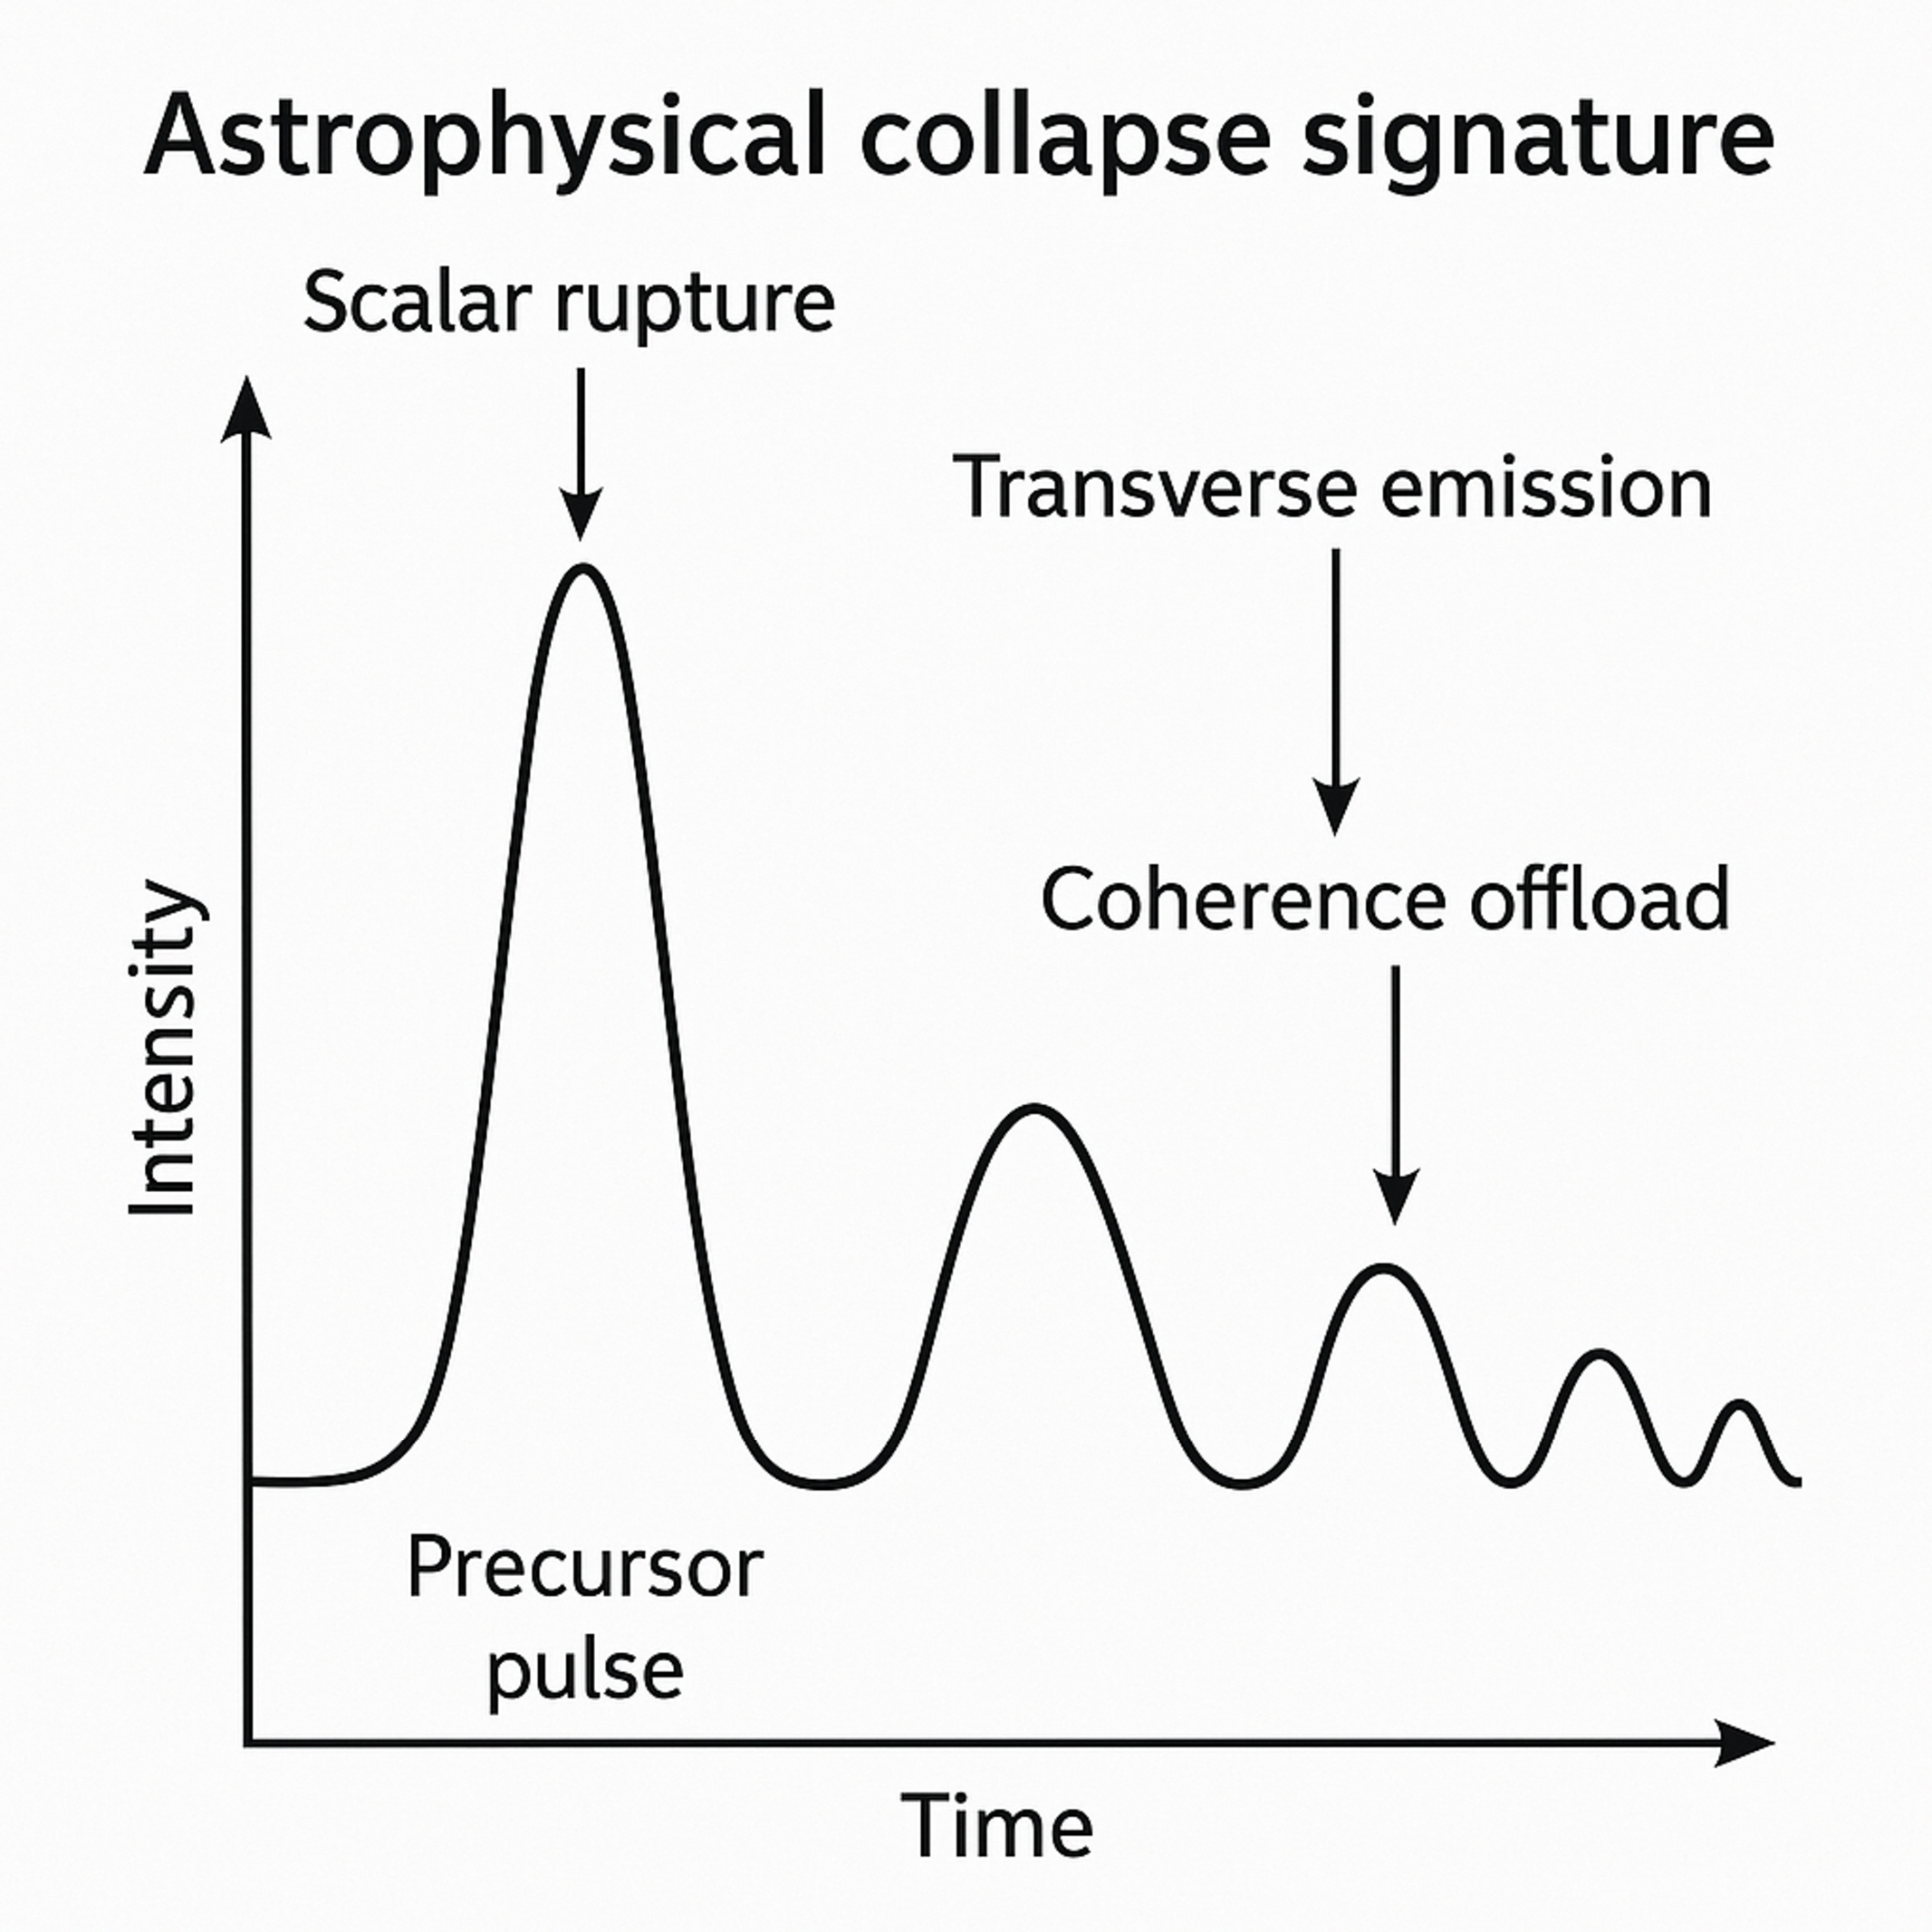
\includegraphics[width=0.85\linewidth]{figures/astrocollapse.pdf}
  \caption{Collapse emission signature predicted by QSD. A sharp precursor pulse marks scalar pacing rupture, followed by a quantized offload train that encodes the internal geometry of the collapsing envelope. This time-asymmetric structure contrasts with classical collapse models and provides a testable emission fingerprint.}
  \label{fig:collapse_signature}
\end{figure}

\subsubsection{Black Hole Precursors and Merger Frustration}

In black hole mergers or near-horizon regimes, QSD predicts coherence trench saturation may lead to merger frustration or scalar offload before full event horizon formation. This opens the possibility for:
\begin{itemize}
  \item \textbf{Pre-merger emissions} that do not align with general relativity’s predictions.
  \item \textbf{Nonlinear delay or recoil patterns} in ringdown waveforms, indicating temporary trench collapse or offload buffering.
  \item \textbf{Energy dissipation without apparent mass loss}, consistent with scalar yield that does not couple to external observers in the electromagnetic domain.
\end{itemize}

Precision gravitational wave observation (e.g., from LIGO, Virgo, or future missions) offers an avenue for testing these predictions through waveform analysis and comparison with classical merger models.

\subsubsection{Laboratory-Scale Analogues}

Though the full Planck-scale collapse process is not reachable in current experimental systems, analog coherence structures may offer indirect paths toward testing substrate behavior:
\begin{itemize}
  \item \textbf{Nonlinear laser compression} in structured media may allow coherence envelope saturation and rupture analogues in photonic systems.
  \item \textbf{Superfluid or BEC phase collapse}, especially in toroidal geometries, may mimic scalar gating, recovery lag, and quantized offload behavior.
  \item \textbf{Fracture dynamics in tensioned lattices} may serve as classical substrate analogs, especially when coupled with phase-controlled energy loading.
\end{itemize}

QSD predicts that in all such systems, there will be a coherence saturation limit beyond which energy cannot be supported in a single domain without triggering a quantized release or phase reset. Identifying such behavior in engineered systems may offer a proof-of-concept for structured yield and coherence threshold mechanics.

\subsubsection{Summary}

Together, these observational and experimental windows offer testable avenues for distinguishing QSD's structural interpretation of Planck energy from traditional models. In each case, the critical prediction is that collapse and emission are not continuous—but quantized, structured, and geometrically constrained. Planck energy becomes, not an abstract boundary, but a concrete and falsifiable limit in the causal substrate dynamics of mass, radiation, and collapse.
%%%%%%%%%%%%%%%%%%%%%%%%%%%%%%%%%%%%%%%%%%%
\subsection{Reinterpreting Planck Units Structurally}

In conventional physics, Planck units---length, time, and energy---are derived through dimensional analysis, combining fundamental constants $\hbar$, $G$, and $c$ into quantities with units of space, time, and energy. These values are often interpreted as heuristic thresholds beyond which classical theories fail, but their physical origin remains undefined. In QSD, these units acquire clear structural interpretations grounded in the substrate’s causal and geometric constraints.

\subsubsection{Planck Length as Coherence Support Radius}

In QSD, the Planck length $L_P$ is not a minimum position scale or a quantum of spacetime. It is the characteristic length scale of a \textit{fully saturated coherence envelope}, below which the substrate cannot maintain stable phase alignment. This coherence length defines the minimal spatial region within which a mass-phase knot can form and persist. Structures smaller than $L_P$ cannot sustain transverse tension under recoverable scalar pacing and therefore fail to stabilize.

\subsubsection{Planck Time as Scalar Recovery Interval}

Planck time $t_P$ is traditionally viewed as the smallest meaningful unit of time. In QSD, it has a causal and functional role:

\begin{equation}
t_P = \frac{L_{\text{coh}}}{c_s}
\end{equation}

This is the minimum time required for scalar recovery to reset a coherence envelope of length $L_{\text{coh}}$. It represents the \textit{substrate's gating interval}: the shortest duration between energy offload events that preserves causal coherence. No energy structure can cycle faster than this interval without disrupting the substrate’s phase continuity. This pacing constraint enforces quantization as a structural necessity.

\subsubsection{Planck Energy as Collapse Limit}

As developed in earlier sections, Planck energy is interpreted in QSD as the maximum energy that can be coherently stored in a region of size $L_{\text{coh}}$ before rupture occurs:

\begin{equation}
E_P = \frac{c_t^4}{G} \cdot L_{\text{coh}} = \hbar \cdot \frac{c_s}{L_{\text{coh}}}
\end{equation}

This expression confirms that $E_P$ is not merely a boundary for theoretical breakdown, but a \textit{structural yield threshold}---the energy limit imposed by substrate geometry and offload pacing. It marks the point at which the envelope can no longer maintain internal waveform symmetry under recoverable conditions.

\subsubsection{Unification Through Substrate Behavior}

In total, QSD unifies the Planck units as expressions of causal substrate behavior:
\begin{itemize}
  \item $L_P$ sets the spatial coherence limit.
  \item $t_P$ sets the temporal pacing limit.
  \item $E_P$ sets the energetic support limit.
\end{itemize}

Each unit reflects the boundary at which the substrate can no longer maintain coherence---not an abstract boundary of knowledge, but a concrete physical limit rooted in geometry, phase stability, and recovery time. These units become falsifiable expressions of causal structure, not theoretical artifacts.

This reinterpretation transforms Planck units from dimensional thresholds into physically meaningful expressions of substrate architecture. They are no longer symbolic placeholders for unknown physics—they are \textit{derived limits on what coherent structure can exist within a conserved and causally gated field}.


%%%%%%%%%%%%%%%%%%%%%%%%%%%%%%%%%%%%%%%%%%
\section{Conclusion}
%%%%%%%%%%%%%%%%%%%%%%%%%%%%%%%%%%%%%%%%%%

In this work, we have reinterpreted Planck energy not as a heuristic boundary derived from dimensional analysis, but as a physically grounded collapse limit arising from the structure of a conserved coherence substrate. Within the Quantum Substrate Dynamics (QSD) framework, $E_P$ defines the maximum energy that can be stably supported within a localized coherence envelope of size $L_{\text{coh}}$ before rupture or offload becomes compulsory. This reinterpretation provides a testable and causally constrained mechanism for quantization, collapse, and emission.

We derived $E_P$ as a function of the transverse coherence propagation rate $c_t$, the scalar recovery rate $c_s$, the curvature compliance $G$, and the coherence envelope geometry:

\begin{equation}
E_P = \frac{c_t^4}{G} \cdot L_{\text{coh}} = \hbar \cdot \frac{c_s}{L_{\text{coh}}}
\end{equation}

This expression reveals that Planck energy is not a fixed threshold but a \textit{contextual structural limit} that varies with coherence geometry and pacing capacity. It marks the point beyond which the substrate can no longer maintain phase stability, leading to scalar emission, rebound structuring, or coherence fracture. Collapse is reframed as a substrate-driven yield event, not a singularity in geometry.

We further showed that this saturation point is deeply linked to the physical interpretations of Planck time and length, unifying all Planck-scale quantities as causal consequences of substrate behavior. In this view, quantization arises from scalar pacing constraints, and energy is limited by the recoverable coherence support of a finite region. These insights lead to falsifiable predictions for burst structure, emission spectra, and rupture thresholds in astrophysical and possibly laboratory systems.

By grounding Planck energy in substrate mechanics, QSD replaces abstract constants with structural causality. The Planck scale becomes the active boundary of coherent structure, not a symbolic boundary of theory. This interpretation provides a foundation for modeling collapse, mass stability, and high-energy emission using causal geometry rather than singular extrapolation. As such, it offers a concrete, testable path forward in understanding both the limits and origins of quantized energy in the physical universe.

%%%%%%%%%%%%%%%%%%%%%%%%%%%%%%%%%%%%%%%%%%
\vspace{6pt} 

%%%%%%%%%%%%%%%%%%%%%%%%%%%%%%%%%%%%%%%%%%
%% optional
%\supplementary{The following supporting information can be downloaded at:  \linksupplementary{s1}, Figure S1: title; Table S1: title; Video S1: title.}

% Only for journal Methods and Protocols:
% If you wish to submit a video article, please do so with any other supplementary material.
% \supplementary{The following supporting information can be downloaded at: \linksupplementary{s1}, Figure S1: title; Table S1: title; Video S1: title. A supporting video article is available at doi: link.}

% Only used for preprtints:
% \supplementary{The following supporting information can be downloaded at the website of this paper posted on \href{https://www.preprints.org/}{Preprints.org}.}

% Only for journal Hardware:
% If you wish to submit a video article, please do so with any other supplementary material.
% \supplementary{The following supporting information can be downloaded at: \linksupplementary{s1}, Figure S1: title; Table S1: title; Video S1: title.\vspace{6pt}\\
%\begin{tabularx}{\textwidth}{lll}
%\toprule
%\textbf{Name} & \textbf{Type} & \textbf{Description} \\
%\midrule
%S1 & Python script (.py) & Script of python source code used in XX \\
%S2 & Text (.txt) & Script of modelling code used to make Figure X \\
%S3 & Text (.txt) & Raw data from experiment X \\
%S4 & Video (.mp4) & Video demonstrating the hardware in use \\
%... & ... & ... \\
%\bottomrule
%\end{tabularx}
%}

\section*{Statements and Declarations}
\subsection*{Funding}  
The author received no financial support for the research, authorship, or publication of this article.
The author has no relevant financial or non-financial interests to disclose.

\subsection*{Competing Interests}  
The author declares no competing interests.

\subsection*{Author Contributions}  
The author solely conceived, developed, and wrote the manuscript, including all theoretical content, references, and formatting.

\subsection*{Data Availability}  
No datasets were generated or analyzed during the current study. All references are publicly available.

\subsection*{Ethical Approval}  
Not applicable.


%%%%%%%%%%%%%%%%%%%%%%%%%%%%%%%%%%%%%%%%%%
%% Optional

%% Only for journal Encyclopedia
%\entrylink{The Link to this entry published on the encyclopedia platform.}

\abbreviations{Abbreviations}{
The following abbreviations are used in this manuscript:
\\

\noindent
\begin{tabular}{@{}ll}
QSD   & Quantum Substrate Dynamics \\
\( c_s \) & Scalar coherence recovery speed (temporal mode) \\
\( c_t \) & Transverse coherence propagation speed (spatial mode) \\
\( L_0 \) & Baseline coherence length at rest \\
\( L_{\text{coh}}(r) \) & Curvature-stretched coherence support length \\
\( \alpha \) & Gravitational curvature constant \\
\( \epsilon \) & Curvature coupling efficiency \\
\( v \) & Velocity relative to substrate \\
\( t_{\text{tick}} \) & Local scalar recovery interval (time tick) \\
\( t_0 \) & Tick duration at rest \\
\( \gamma \) & Lorentz factor (inherited form from conservation triangle) \\
GPS  & Global Positioning System \\
SR   & Special Relativity \\
GR   & General Relativity \\
\end{tabular}
}



%%%%%%%%%%%%%%%%%%%%%%%%%%%%%%%%%%%%%%%%%%
%% Optional
\appendixtitles{no} % Leave argument "no" if all appendix headings stay EMPTY (then no dot is printed after "Appendix A"). If the appendix sections contain a heading then change the argument to "yes".
\appendixstart
\appendix
%%%%%%%%%%%%%%%%%%%%%%%%%%%%%%%%%%%%%%%%%%%%%%%
\section[\appendixname~\thesection]{}
\subsection[\appendixname~\thesubsection]{Connection to Other QSD Papers}
%%%%%%%%%%%%%%%%%%%%%%%%%%%%%%%%%%%%%%%%%%%%%%

This paper builds upon foundational results developed in previous works on Quantum Substrate Dynamics (QSD), especially those addressing the structural origins of quantization, coherence geometry, and gravitational coupling.

\subsubsection{Planck’s Constant and Coherence Derivation}
In the earlier paper on the physical origin of Planck’s constant, $\hbar$ was derived as a structural offload quantity:

\begin{equation}
\hbar = \frac{c_t^4}{c_s} \cdot \frac{L_{\text{coh}}^2}{G}
\end{equation}

This expression reframed $\hbar$ not as an axiomatic quantum of action, but as a consequence of substrate geometry, causal pacing, and curvature compliance. The present work draws directly on this result to invert the relation and express $G$ structurally, leading to the geometric derivation of the Planck energy:

\begin{equation}
E_P = \frac{c_t^4}{G} \cdot L_{\text{coh}} = \hbar \cdot \frac{c_s}{L_{\text{coh}}}
\end{equation}

\subsubsection{Coherence Envelopes and Mass Stability}
The companion paper on coherence envelopes introduced the concept of $L_{\text{coh}}$ as the spatial domain required to support a stable phase-locked mass structure. There, $L_{\text{coh}}$ defined:
\begin{itemize}
  \item The boundary of coherent phase alignment,
  \item The minimum offload pacing interval,
  \item The energy limit for reversible structure within a mass-phase knot.
\end{itemize}

The current paper extends this by establishing the energy saturation point of such an envelope, linking $E_P$ directly to collapse onset and structured rupture behavior.

\subsubsection{Mergers and Trench Collapse Phenomena}

In prior work on merger frustration and TIGBs (trench-induced gamma bursts), QSD predicted that gravitationally bound systems approaching trench saturation would exhibit burst emission or structural instability prior to traditional merger. The Planck energy threshold derived here provides a physical basis for these behaviors: it defines the energy ceiling beyond which coherent envelopes can no longer combine without violating scalar pacing constraints.

In regions where multiple coherence envelopes approach saturation simultaneously, strain coupling may occur through overlapping phase-tension gradients. These adjacent $L_{\text{coh}}^3$ domains may influence each other's stability, potentially triggering synchronized rupture or cascade failure. QSD predicts the existence of \textit{collapse networks}—structured regions in which local yield events propagate nonlinearly through coherence-linked substrate domains. Such dynamics are most likely to appear in merger zones, shockfront boundaries, or lattice-like astrophysical systems where scalar pacing and geometric strain are tightly coupled.


\subsubsection{Unified Interpretation of Quantization and Collapse}
Taken together, these papers form a triangulated theory of structure in QSD:
\begin{enumerate}
  \item $\hbar$ arises from minimal coherence offload,
  \item $G$ reflects curvature compliance,
  \item $E_P$ defines structural failure under excess tension,
  \item $L_{\text{coh}}$ provides a common geometric substrate.
\end{enumerate}

This work therefore completes a key part of the QSD program: establishing the physical, falsifiable, and quantized nature of collapse behavior from first principles rooted in coherence geometry.

Readers interested in deeper derivations of these relationships are referred to:
\begin{itemize}
  \item \textit{QSD Planck’s Constant Derivation} [QSD\_Plancks\_Pre.pdf]
  \item \textit{QSD Coherence Envelope Geometry} [QSD\_Lcoh\_PrePrint.pdf]
  \item \textit{QSD Trench Collapse and Merger Frustration} [QSDMergers.pdf]
\end{itemize}

%%%%%%%%%%%%%%%%%%%%%%%%%%%%%%%%%%%%%%%%%%%%%%

%%%%%%%%%%%%%%%%%%%%%%%%%%%%%%%%%%%%%%%%%%%%%%%
%\section[\appendixname~\thesection]{}
%\subsection[\appendixname~\thesubsection]{APP B}
%%%%%%%%%%%%%%%%%%%%%%%%%%%%%%%%%%%%%%%%%%%%%%%

%\subsubsection{SUB B}

%%%%%%%%%%%%%%%%%%%%%%%%%%%%%%%%%%%%%%%%%%
%\isPreprints{} % If the paper is ``preprints'', please uncomment this parenthesis.
%\printendnotes[custom] % Un-comment to print a list of endnotes

\reftitle{References}

% Please provide either the correct journal abbreviation (e.g. according to the “List of Title Word Abbreviations” http://www.issn.org/services/online-services/access-to-the-ltwa/) or the full name of the journal.
% Citations and References in Supplementary files are permitted provided that they also appear in the reference list here. 

%=====================================
% References, variant A: external bibliography
%=====================================
% \bibliography{your_external_BibTeX_file}

%=====================================
% References, variant B: internal bibliography
%=====================================

% ACS format
\isAPAandChicago{}{%
\begin{thebibliography}{999}
% Reference 
\bibitem{bush2025}
\textbf{Preprint.} Bush, M. (2025). Quantum Substrate Dynamics (QSD): A Relativistic Field Model of Emergent Mass, Inertia and Gravity. \textit{Preprints}, 2025060988. \url{https://doi.org/10.20944/preprints202506.0988.v1}
% reference
\bibitem{bush-planck-2025}
\textbf{Preprint.} Bush, M. (2025). Planck’s Constant Physically Derived Through Quantum Substrate Dynamics: A Mode-Ratio and Offload-Based Origin for Quantization and Temporal Structure. \textit{Preprints}, 2024010211. \url{https://doi.org/10.20944/preprints202401.0211.v1}

% Reference 
\bibitem{planck1901}
\textbf{Journal article.} Planck, M. (1901). On the Law of Distribution of Energy in the Normal Spectrum. \textit{Annalen der Physik}, 4(553–563). \url{https://doi.org/10.1002/andp.19053221004}
% Reference 
\bibitem{einstein1905} 
\textbf{Journal article.} Einstein, A. (1905). On the electrodynamics of moving bodies. \textit{Annalen der Physik}, 322(10), 891–921. \url{https://doi.org/10.1002/andp.19053221004}
% Reference 
\bibitem{einstein1915} 
\textbf{Journal article.} Einstein, A. (1915). The field equations of gravitation. \textit{Sitzungsberichte der Preussischen Akademie der Wissenschaften}.
% Reference 
\bibitem[Ashby(2003)]{ashby-gps}
Ashby, N. Relativity in the Global Positioning System. {\em Living Rev. Relativ.} {\bf 2003}, {\em 6}, 1--50. \url{https://doi.org/10.12942/lrr-2003-1}.
% Reference
\bibitem[Bailey et al.(1977)]{bailey-muon}
Bailey, J.; Borer, K.; Combley, F.; Drumm, H.; Krienen, F.; Picasso, E.; von Ruden, W.; Farley, F.J.M.; Field, J.H. Measurements of relativistic time dilatation for positive and negative muons in a circular orbit. {\em Nature} {\bf 1977}, {\em 268}, 301--305. \url{https://doi.org/10.1038/268301a0}.
% Reference
\bibitem{boyd2008}
\textbf{Book.} Boyd, R.W. (2008). \textit{Nonlinear Optics} (3rd ed.). Academic Press.
% Reference
\bibitem{zurek2003}
\textbf{Journal article.} Zurek, W.H. (2003). Decoherence, Einselection, and the Quantum Origins of the Classical. \textit{Reviews of Modern Physics}, 75(3), 715–775. \url{https://doi.org/10.1103/RevModPhys.75.715}
% Reference
\bibitem{duff2002}
\textbf{Journal article.} Duff, M.J.; Okun, L.B.; Veneziano, G. (2002). Trialogue on the number of fundamental constants. \textit{Journal of High Energy Physics}, 2002(03), 023. \url{https://doi.org/10.1088/1126-6708/2002/03/023}


\end{thebibliography}
}

% Chicago format (Used for journal: arts, genealogy, histories, humanities, jintelligence, laws, literature, religions, risks, socsci)
\isChicagoStyle{%
\begin{thebibliography}{999}
% Reference 1
%\bibitem[Aranceta-Bartrina(1999a)]{ref-journal}
%Aranceta-Bartrina, Javier. 1999a. Title of the cited article. \textit{Journal Title} %6: 100--10.
% Reference 2

\end{thebibliography}
}{}

% APA format (Used for journal: admsci, behavsci, businesses, econometrics, economies, education, ejihpe, games, humans, ijfs, journalmedia, jrfm, languages, psycholint, publications, tourismhosp, youth)
\isAPAStyle{%
\begin{thebibliography}{999}
% Reference 1
%\bibitem[\protect\citeauthoryear{Azikiwe \BBA\ Bello}{{2020a}}]{ref-journal}
%Azikiwe, H., \& Bello, A. (2020a). Title of the cited article. \textit{Journal Title}, \textit{Volume}(Issue), 
%Firstpage--Lastpage/Article Number.

\end{thebibliography}
}{}

% If authors have biography, please use the format below
%\section*{Short Biography of Authors}
%\bio
%{\raisebox{-0.35cm}{\includegraphics[width=3.5cm,height=5.3cm,clip,keepaspectratio]{Definitions/author1.pdf}}}
%{\textbf{Firstname Lastname} Biography of first author}
%
%\bio
%{\raisebox{-0.35cm}{\includegraphics[width=3.5cm,height=5.3cm,clip,keepaspectratio]{Definitions/author2.jpg}}}
%{\textbf{Firstname Lastname} Biography of second author}

% For the MDPI journals use author-date citation, please follow the formatting guidelines on http://www.mdpi.com/authors/references
% To cite two works by the same author: \citeauthor{ref-journal-1a} (\citeyear{ref-journal-1a}, \citeyear{ref-journal-1b}). This produces: Whittaker (1967, 1975)
% To cite two works by the same author with specific pages: \citeauthor{ref-journal-3a} (\citeyear{ref-journal-3a}, p. 328; \citeyear{ref-journal-3b}, p.475). This produces: Wong (1999, p. 328; 2000, p. 475)

%%%%%%%%%%%%%%%%%%%%%%%%%%%%%%%%%%%%%%%%%%
%% for journal Sci
%\reviewreports{\\
%Reviewer 1 comments and authors’ response\\
%Reviewer 2 comments and authors’ response\\
%Reviewer 3 comments and authors’ response
%}
%%%%%%%%%%%%%%%%%%%%%%%%%%%%%%%%%%%%%%%%%%
\PublishersNote{}
%\isPreprints{} % If the paper is ``preprints'', please uncomment this parenthesis.
\end{document}

